%%%% début de la page
\teteSndMouv

%%%% titre
\numeroActivite{6}
\titreActivite{Poids et interaction gravitationnelle}

%%%% objectifs
\begin{objectifs}
  \item Comprendre le lien entre la force d'interaction gravitationnelle et le poids
\end{objectifs}


%%
\begin{doc}{Force d'interaction gravitationnelle}{doc:A6_interaction_gravitationnelle}
  \chevron Tous les corps qui possèdent une masse s’attirent entre eux : c’est l’attraction gravitationnelle.

  \begin{importants}
    On modélise l'attraction gravitationnelle exercée par le corps $A$ sur le corps $B$ par une force représentée par un vecteur $\vvFAsurB$ :
    
    \vspace*{-12pt}
    \begin{wrapfigure}[6]{r}{0.4\linewidth}
      \vspace*{-20pt}
      \begin{tikzpicture}
  % corps A
  \tikzCercle[gray!50!white] (0, 0) {20}
  \tikzLabel(-1.2, 0) {$m_A$}
  \tikzPointLabel(0,0) {$A$}
  % corps B
  \tikzCercle[gray!50!white] (4, 2) {20}
  \tikzLabel(2.8, 2) {$m_B$}
  \tikzPointLabel(4, 2) {$B$}
  % force et distance
  \tikzVecteur(4, 2) (-1.75, -0.875) {$\vvFAsurB$} [left]
  \tikzVecteur*(0.5, -1) (4, 2) {}
  \tikzLabel(2.5, -0.5) {$d$}
\end{tikzpicture}
    \end{wrapfigure}

    \phantom{b}
    \begin{listePoints}
      \item \important{Point d'application} : centre du corps $B$
      \item \important{Direction} : la droite $AB$.
      \item \important{Sens} : de $B$ vers $A$ (force attractive).
      \item \important{Valeur} : 
    \end{listePoints}
    \begin{center}
      $\FAsurB = G\times \dfrac{m_A \times m_B}{d^2}$
    \end{center}
      
    Dans la formule de la valeur de la force, les masses s'expriment en kilogramme (\unit{\kg}),
    la distance en mètre (\unit{\m}) et
    la \important{constante universelle de gravitation $\mathbf{G}$} en newton mètre carrée par kilogramme carrée (\unit{\newton \m\squared \per\kg\squared}).
    Sa valeur (à connaître) est 
    \begin{center}
      $G = \qty{6,67e-11}{\newton \m\squared \per\kg\squared}$
    \end{center}
  \end{importants}
\end{doc}

\begin{doc}{La planète Terre}{doc:A6_terre}
  La Terre est la troisième planète du système solaire.
  En première approche, on peut considérer que la Terre est une boule de rayon $R_T = \qty{6,37e6}{\m}$
  et de masse $M_T = \qty{5,97e24}{\kg}$.
\end{doc}

%%%%
On cherche à calculer la force d'interaction gravitationnelle qu'exerce la Terre sur un objet de masse $m$ \important{à la surface de la Terre}.
  
\begin{center}
  \begin{tikzpicture}
    % Terre et Objet
    \tikzCercle[couleurSec!30] (0, 0) {60} [couleurSec]
    \tikzLabel(0, 0) {$T$}
    \tikzLabel(2.12, 0) {Objet} (3, 0)
    % Rayon de la Terre
    \tikzVecteur*(0, 0) (-0.54, -2.05) {}
    \tikzLabel*(0.3, -1) {$R_T$}
  \end{tikzpicture}
  
  \legende{Représentation de la Terre avec un objet à sa surface}
\end{center}


\question{
  Donner la formule littérale de la valeur de la force d'interaction gravitationnelle 
  $F_{T/objet}$ qu'exerce la terre sur l'objet.
}{
  \begin{equation*}  
    F_{T/objet} = G\times \dfrac{m \times M_T}{R_T^2}
  \end{equation*}
}[3]

\newpage
\question{
  Rappeler la formule littérale du poids $P$ que la Terre exerce sur un objet de masse $m$ sur Terre.
  Rappeler la valeur de $g$
}{
  \begin{equation*}
    P = m \times g
  \end{equation*}
  g = \qty{9.81}{\newton}
}[3]

\question{
  Dans l'expression de $F_{T/objet}$, on va regrouper tous les termes qui sont constant sur Terre et les noter $g$.
  Donner la formule littérale de $g$ en fonction de $M_T$, $R_T$ et de $G$.
}{
  \begin{equation*}  
    F_{T/objet} = G\times \dfrac{m \times M_T}{R_T^2}
    = m \times \dfrac{G \times M_T}{R_T^2}
    = m \times g
  \end{equation*}
  Et donc 
  \begin{equation*}
    g = \dfrac{G \times M_T}{R_T^2}
  \end{equation*}
}[3]

\question{
  Calculer la valeur numérique de $g$. 
  En déduire le lien entre le poids $P$ et $F_{T/objet}$.
}{
  \begin{equation*} 
    g = \dfrac{G \times M_T}{R_T^2}
    = \dfrac{\qty{6,67e-11}{\newton \m\squared \per\kg\squared} 
        \times \qty{5.97e24}{\kg}}
      {(\qty{6.37e6}{\m})^2}
    = \qty{9.813}{\newton\per\kg}
  \end{equation*}
  On voit donc que le poids est simplement l'interaction gravitationnelle de la Terre sur un objet à la surface de la Terre.
}[5]